\documentclass[11pt, twocolumn]{article}

% GRAPHICS
\usepackage{float}
\usepackage{graphicx}
\usepackage{subcaption}

% HYPERLINKS
\usepackage{hyperref}

% DOCUMENT PADDING AND MARGINS
\usepackage{titlesec}
\usepackage[margin=0.8in]{geometry}
%\setlength{\parskip}{\baselineskip}%
%\setlength{\parindent}{0pt}
\titlespacing*{\section}{0pt}{2ex}{0ex}
\titlespacing*{\subsection}{0pt}{2ex}{0ex}
\titlespacing*{\subsubsection}{0pt}{2ex}{0ex}

% COMMENTING
\usepackage{comment}

% MATH FONTS
\usepackage{amsmath}


\begin{document}

% TITLE
\title{Autonomous Quadrotor Landing on a Moving Platform}
\author{Stan Brown \& Chris Choi}
\date{}
\maketitle


\section{Introduction}

The idea of quadrotor has been explored by several companies and researchers since quadrotors became a popular alternative to fixed wing and single rotor aircraft (DJI auto landing, Pixhawk, make a reference). However most of these methods usually assume that the landing zone is static and that there is very little wind or disturbances. In cases of high wind or a rapidly moving platform, which from the quadrotor's reference frame can be be though of as nearly equivalent cases, normal autonomous landing procedures will likely fail. 

Over the years there has been been at least some interest in the problem of landing a quadrotor on a moving platform and there have been at least 5 academic publications on the topic \cite{Lee2012, Kim2014, Voos2010, Friis2009, Ling2014, Herisse2012}. The problem has been explored from a fairly wide range of approaches. 

Possible applications for this work include autonomous landing on a boat in high wind conditions, landing on a charging platform and more.

The major challenge with autonomous precision landing is the difficulty of obtaining a reliable estimate of the landing target relative to the quadrotor, the landing target can often go out of the camera's field of view causing the quadrotor to lose track of the target, other vision based artifacts that include lighting, lens distortion, color, etc.


\section{Related Work}
The challenging of autonomous landing can be categorized into three distinct parts. First, the quadrotor must sense or detect the landing target to obtain positional estimates relative to the quadrotor. Secondly, the quadrotor must plan its rendezvous trajectory with the landing target. Third and finally, the quadrotor must apply a set of controller commands to approach the platform, matching both speed and heading on the approach and land on the moving target. 

\subsection{Perception and State Estimation}
For perception existing solutions use a variety of simple to complex techniques. In \cite{Kim2014} a basic color threshold technique was to identify the landing target, while \cite{Herisse2012} used optical flow in images captured on board the quadrotor to obtain necessary relative information for control. 

\subsection{Planning}
In the literature we reviewed, rendezvous planning was neglected as it was assumed that quadrotor has a clear view of its landing target. Most authors tend to focus on the detection and estimation of the quadrotor's pose relative to the target and maintaining an accurate estimation throughout the landing procedure which is mostly handled by a series of control loops.

\subsection{Control}
A comparison between a PID and Linear Quadratic Control (LQC) was explored in \cite{Friis2009}. However the authors admit, even though LQC performed slightly better than the PID controller the difference was minor and may be attributed to the additional time spent tuning the LQC. In \cite{Herisse2012} a PID controller was developed to land on a oscillating platform in the vertical direction with no lateral movement. While interesting, the solution took over 1 minute to transition from hovering over the landing pad to landing. Additionally the experiments did not seem to account for pitch or roll of the platform.  

\section{Methodology}

\section{Hardware}
\subsection{Quadrotor}
For the hardware, we have chosen to reuse equipment that is readily available to us in the Wave Lab. For the quadrotor we have been using the DJI F450 quadrotor frame, Emax 2213-935KV motors with complimentary 1045R propellers, Thunder Power lipo 11.1V 4200mah battery, DJI E310 420S 20A electronic speed controller and Pixhawk v2.4 as our flight controller.

\begin{figure}[H]
	\centering
	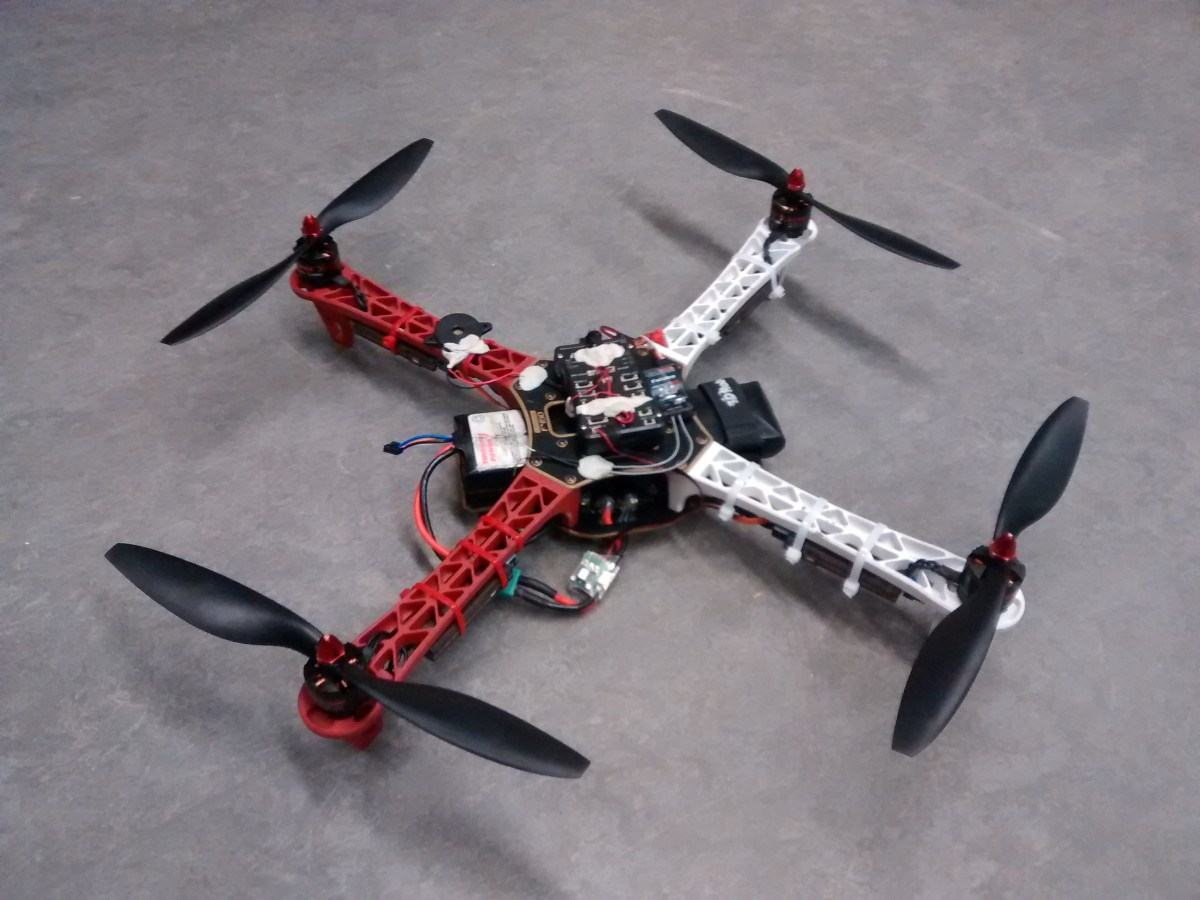
\includegraphics[width=0.8\linewidth]{images/quadrotor.jpg}
	\caption{DJI F450 with Pixhawk v1.5}
\end{figure}

\subsubsection{Onboard Autonomous Control System}
In terms of onboard autonoumos control, we have decided to use the Odriod XU4 due to its size and processing power available, and a Logitech C270 HD webcam as our vision sensor. One problem we may face very soon is the narrow field of view and relatively low frame rate (25Hz) the logitech webcam has. We will be keeping our options open, and plan on replacing the logitech webcam with a Ximia xiQ USB3 camera with a wide angle lens in the near future.

\subsection{Vision Capture}
Firefly camera

\subsubsection{Pixhawk Firmware - PX4}
As mentioned in the hardware section, we have had numerous issues with regards to using the software suite for the Pixhawk Flight Controller, as well as the PX4 firmware itself. There are many instances where we could not explain the instability of the quadrotor during flight, many of which lead to costly crashes, but we believe through these experiences we have developed a procedure to lower the risk for such instances from happening often.

\subsubsection{Odriod to Pixhawk Communication}
For our autonomous system to control the quadrotor directly, the Odriod has to be able to communicate with the Pixhawk, this is where \verb|mavros| (ROS package) comes into play. Mavlink is a popular UAV communication protocol between UAV and ground control softwares, \verb|mavros| creates a mavlink ROS node to enable developers to monitor and issue mavlink commands with ease. We have successfully used mavros to arm and disarm Pixhawk (tested), in the near future we should be able to send velocity/attitude commands to control the quadrotor.

\subsubsection{AprilTag}
On the landing target from we have successfully calibrated the Logitech webcam and used the Apriltag library to obtain a pose estimate, and have manually verified the estimates are accurate, for distance the error is $\pm 1$cm. We have also successfully implemented the ability to identify two different apriltags of different sizes (see Fig~\ref{fig:apriltag}), pose estimates from both apriltags are equal.

Next is to workout how to transform the measurements from the pose estimates of the apriltags in relation to the quadrotor's body frame.


\subsection{Quadrotor Control}
In reviewing prior work, a reoccurring problem lies in the difficulty in maintaining an accurate pose estimation between the quadrotor and the landing target throughout the entire manoeuvre. As the quadrotor approaches the landing target, the target often goes beyond the camera's field of view, causing camera based navigation techniques to fail. Furthermore, in certain conditions the tilt angle of the quadrotor could cause difficulty in maintaining a visual on the landing pad for a downward facing or fixed camera. 

To address both of these issues, we propose a novel solution utilizing an nested apriltags which we term inception apriltag. We will replicate the experiment performed by \cite{Ling2014}, where we assume the quadrotor already has a visual of the landing platform. We aim to implement a series of controllers for the approach and landing of the quadrotor to the moving landing platform.

\subsection{Measurement and State Estimation}

One of the major challenges when using AprilTags on a robot that has limited computational power, such as a quadrotor, is the rate at which the AprilTag library can compute the state. This problem is exacerbated when using larger image sizes as the computational time of the AprilTag software appears to grow at least exponentially as shown in (add a figure here). This problem was also noted in the work of \cite{Ling2014} and he addressed the issue by reducing the brightness of the image so that majority of the image is black except for the april tag. An example of this implementation is shown in figure (Kevins image). This allowed Ling \cite{Lee2012} to calculate states at a rate of approximatly 10 - 15 fps but it came at the cost of requiring the brightness parameters to be set ahead of time and also removed a lot of the robustification that is provided in the standard AprilTag library.

In this work, the slow rate of state estimation was addressed using a novel method where the image size and calibration parameters are set depending on the current distance between the quadrotors position relative to the landing pad. 

\subsection{Adaptive Image Preprocessing}

As discussed previously, the low rate of the AprilTag library when processing images of 640 by 480 pixels results in an update rate of approximately 3 to 5 fps on a Snapdragon 8 core processor, which is to low to be used effectively in a PID control loop. Building on the work of Ling, who noted that higher update rates were possible using AprilTags when the majority of the image is filled with black pixels, a set of image preprocessing methods were developed to maximize the update rate of the AprilTag library. 

\subsubsection{Adaptive Image Windowing}

If one assumes that the quadrotor does not move to fast, there is relativity low rotation between image captures, and that the image update rate is quite fast (60 fps in this implementation), then the location the AprilTag in the following image can be estimated based off of the location it was last observed in the previous image. Therefore whenever an AprilTag is measured in an image, a bounding box around the AprilTag is calculated and then used in the following image to black out the protions of the image where the AprilTag is unlikely to be. An example of this implementation is highlighted in Figure (Adptive windowing).


While the adaptive windowing procedure works well for when the AprilTag observed at a distance, where they do not take up a significant portion of the image, it begins to fail when the quadrotor approach the landing pad as the observed size of AprilTag begins to become larger and larger in the  image. This leads to the processing time of the AprilTags to increase as the quadrotor gets closer, which is a major issue as in these cases a higher update rate is actually required. In cases where the AprilTag is not observed in the expected location (bounding box), the size of the bounding box is set to the size of the image and the entire image is processed. 

\subsubsection{AprilTag Inception}
 In order to be used for landing, the AprilTag attached to the landing pad must be relatively larger so that it can be detected from a distance of at least 15 meters which from our experience means the AprilTag must be at least 50 cm by 50 cm in size. The large size of the AprilTag becomes a major issue during the final portion of the landing procedure as the AprilTag image will both appear quite large in the captured image which causes to the Adaptive Windowing Procedure outlined above to become ineffective. Furthermore close proximity to the AprilTag also grealy increases the chance that a portion of the AprilTag will be located outside of the captured image, causing no state estimation to be provided at the critical stages of landing. 
 
To address both the decreasing state update rate as a function of proximity and reduce the probablity of losing site of the AprilTag during landing a secondary AprilTag is embedded in the larger AprilTag. This secondary AprilTag is assigned different family id, and is placed in the center of a primary AprilTag. Whenever the secondary AprilTag is captured in the image, the adaptive windowing method is set to track only the secondary AprilTag rather than the larger one, which reduces the portion of the image that must be processed in with each image capture. An example of this procedure is highlighted in Figure \ref{fig:apriltagInception}.

\begin{figure}[H]
	\centering
	\begin{subfigure}[b]{0.45\linewidth}
		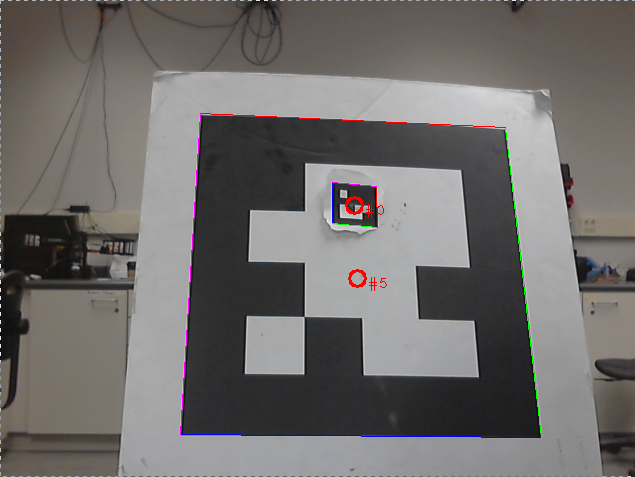
\includegraphics[width=\textwidth]{images/apriltags_1.png}
		\caption{2 Apriltags Detected}
	\end{subfigure}
	\begin{subfigure}[b]{0.45\linewidth}
		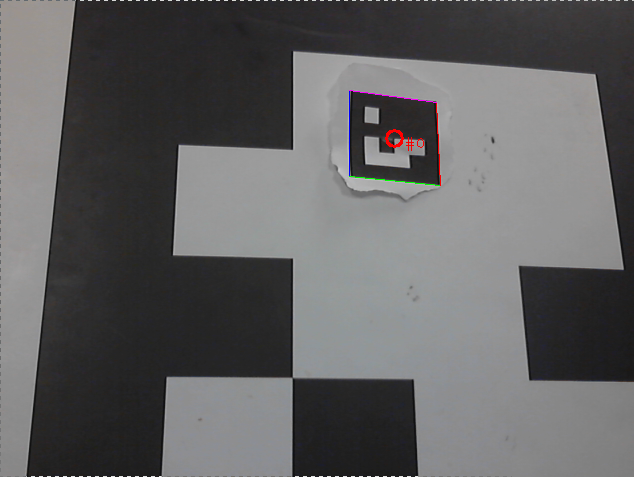
\includegraphics[width=\textwidth]{images/apriltags_3.png}
		\caption{1 Apriltag Detected }
	\end{subfigure}
	\caption{Apriltag Inception - To mitigate the FOV problem assocaited with }
	\label{fig:apriltagInception}
\end{figure}

\subsubsection{Adaptive Image Down-sampling}
It was also noted that the image could be greatly down sampled as well if the quadrotor approaches the landing pad as not as many pixels are required to calculated the location and state of the AprilTag in the image. Therefore 3 image sampling sizes were also introduced into the code which sub-sample the image to 160 by 140 pixels and 320 by 280 (half and quarter resolution) when the distance between the camera and the AprilTag is less than 1.5 and 3 meters respectively. If the camera is further than 3 meters from the AprilTag the native resolution of 640 by 480 is used. This change only affected the image processing time when the quadrotor is within 3 meters of the quad and has the desired effect of increasing the rate of AprilTag process.

In order to use this down sampling effectively without corrupting the AprilTag estimations, 3 camera calibration files were also computed at the normal, half and quarter camera resolutions. The calibration file passed to the AprilTag library during the state estimation proccedure is selected based on what the current camera resolution is set at. 



\section{Results}


\subsubsection{Detection Delay}
\begin{equation}
    t_{\text{capture}} = t - \delta t_{\text{camera}} + \delta t_{\text{detection}}
\end{equation}


\bibliography{report}{}
\bibliographystyle{ieeetr}

\end{document}
